

\subsubsection*{Outline}
As mentioned in the introduction, cost-benefit analysis of water interventions has largely been used on small scales. 
Thus, we undertook an approach that estimates and automates the use of this method.
This approach was based on the qualitative outline given by the World Health Organization in the book "Valuing Water, Valuing Livelihoods."
Essentially, this method calculates the ratio of benefits over costs in the form of Disability Adjusted Life Years gained over US Dollars.

\begin{equation}
\begin{aligned}
& \begin{matrix} \underline{\text{Years Gained}} \\ \text{Dollars} \end{matrix}
\end{aligned}
\end{equation}

Where Disability Adjusted Life Years are defined as:

\begin{equation}
\begin{aligned}
& \text{DALY} = (T \times n) + [(m \times d) + (D \times L)]\\
& T = \text{Travel time to water}\\
& n = \text{Trips to water per year}\\
& m = \text{Number of cases of diarrhea}\\
& d = \text{Days sick per case}\\
& D = \text{Death by diarrhea per year}\\
& L = \text{Average life expectancy}\\
\end{aligned}
\end{equation}

These variables were computed in the assigned survey clusters and their estimation required survey date, standard industry values, and statistical inference.
The following is an outline the techniques used to calculate the cost and benefit of water system interventions.
First, we state the objective function, which is to be maximized. 
Second, we explain each of the variables in the function in its own subsection.

\subsubsection*{Objective Function}
Let $X = \{X_1,X_2,X_3,...,X_n\}$ be the survey cluster locations and $y = \{y_1,y_2,y_3,y_4\}$ be the possible water interventions in a cluster.
These are defined more specifically as:
\begin{equation}
\begin{aligned} 
& y_1 = \text{Distribution of Chlorine Filters}\\
& y_2 = \text{Hand Dug Well}\\
& y_3 = \text{Drilled Well}\\
& y_4 = \text{Communal Standpipe}\\
\end{aligned}
\end{equation}

Then, the objective statement for each $X_i$ is formulated as: %include per household somehow

\begin{equation}
\begin{aligned}
& \underset{y}{\text{maximize}}
& & \frac{T_y + S_y}{P_y}  \\
\end{aligned}
\end{equation}
\begin{equation*}
\begin{aligned}
& T_y = \text{Travel Time Gained from } y_i \\
& S_y = \text{Illness and Death Time Gained from } y_i \\
& P_y = \text{Cost of Intervention } y_i \\
\end{aligned}
\end{equation*}

\subsubsection*{Travel Improvements}
The travel time gained is only estimated for $y_2,y_3,y_4$, because these constitute the creation of a new water source.
In order to consider the effects of the location of the intervention on the benefit it contributes, mathematical and statistical techniques were used.
This also served the purpose of "filling in the gaps" of exact GPS locations of survey participants.
[Make sure data section covers this gap]
First, the entire area of the country was split up into subregions by using a Voronoi diagram.
For a full explanation of the method of Voronoi partitioning, the reader can consult ("Voronoi Diagrams – A Survey of a Fundamental Geometric Data Structure". ACM Computing Surveys. 23 (3): 345–405.  doi>10.1145/116873.116880 ) .
This mathematical technique partitions an area into sections based on the GPS location of cluster centers. %include Voronoi equation
The area of each shape was then computed by truncated the sections with the region boundaries and using Gauss' Area Formula. %include shoelace formula

%%% Include picture of sample Voronoi shapes in country or region boundaries %%%
\begin{figure}[h]
    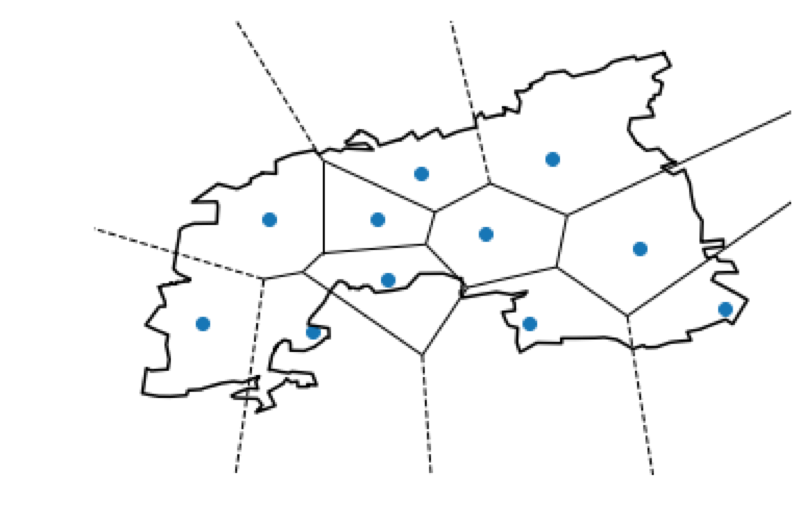
\includegraphics[width=\linewidth]{figures/voronoi.png}
    \caption{Sample Voronoi diagram within region.}
    \label{fig:voronoi}
\end{figure}

With this area found, a square shape was created with the same area as the section in the Voronoi diagram. Then, using a uniform random number generator, several population centers were chosen. 
After, the location of each surveyee was estimated by offsetting their coordinates from one of the population centers. 
Finally, individuals were allocated to the coordinates chosen for each surveyee based upon their reported distance from a water source (Figure 1). 
Those who lived closer to a water source were assumed to live closer to a population center.   
Another assumption made implicitly through using this method was that most surveyees live in clumps or population centers.

%%% Include picture of square with points scattered %%%
\begin{figure}[h]
    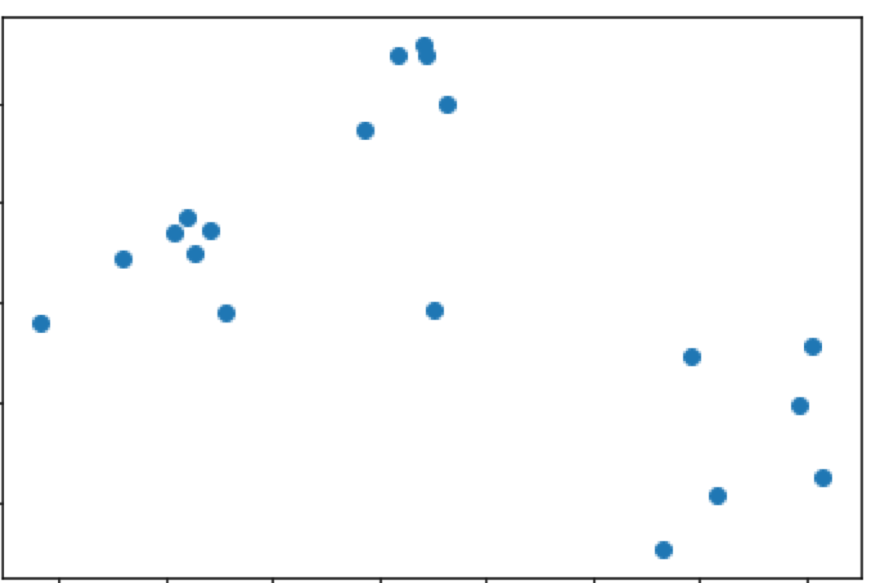
\includegraphics[width=\linewidth]{figures/clusters.png}
    \caption{Sample of cluster distribution per iteration.}
    \label{fig:clusters}
\end{figure}

A water source was then figuratively placed in the middle of the square and each record was reviewed to see if it had an improved access to water, and what the magnitude of the improvement was.
This process was performed $G$ times, and the results were recorded as $a_j$ for impact status of an intervention on household $j$ and $b_j$ for the magnitude of the impact on that household.

%%%%%%%%%%%%%%%%%%%%%%%%
\begin{equation*}
\begin{aligned}
& a_j = \{a_{j1},a_{j2},...,a_{jG}\}\\\\
& a_{jg} =
\left\{
\begin{array}{ll}
      0 & \text{if impact}\\
      1 & \text{if no impact} \\
\end{array}
\right.\\\\
& b_j = \{b_{j1},b_{j2},...,b_{jG}\}\\\\
& b_{jg} =
\left\{
\begin{array}{ll}
      t_{\text{new}} - t_{\text{prev}} & \text{if g had impact} \\
      0 & \text{if g had no impact}\\
\end{array}
\right.
\end{aligned}
\end{equation*}

After $G$ iterations, the estimated probability that each record would be affected by a given intervention was given by:
\begin{equation*}
\frac{1}{G} \sum_{j=1}^{j=G} a_j
\end{equation*}
The approximate number of households affected in an intervention was given by:
\begin{equation*}
a = \sum_{j=1}^{J} \sum_{g=1}^{G} a_{jg}
\end{equation*}
The average total impact that the intervention had on all of these households was estimated as as
\begin{equation*}
T_y = \frac{\sum_{j=1}^{J} \sum_{g=1}^{G} b_{jg}}{G}
\end{equation*}

The improvement a given intervention allotted to citizens through the reduction of travel time from retrieval of water was quantified by this method.

\subsubsection*{Illness and Death Improvements}
In addition to reducing the travel time to collect water, all listed interventions were assumed to give an improvement in health by reducing the cases of diarrhea in a country. 
This reduction in cases was calculated in terms of relative risk of sickness, and was based in large part upon the the findings of ******** and *********.
The original sickness rate was calculated via survey data.
Then, the amount of cases of sickness that the intervention prevented was multiplied by the average amount of healthy life years that were saved from this intervention. A relative risk of $0$ means that there are no more cases of diarrhea after the intervention while $1$ would mean that the intervention has no effect.

\begin{equation*}
\begin{aligned}
& r_i = \text{relative risk for } y_i \\
& N = \text{number of cases before intervention} \\
& k = \text{time conversion factor to years} \\
& D = \text{3 days of sickness per case} \\
& LE  = \text{life expectancy} \\
& AD = \text{average age of death from diarrhea} \\
& PD = \text{proportion of diarrhea cases that end in death} \\
& DALY_{sickness} = k \times (1-r_i) \times N \times d \\
& DALY_{death} = (1-r_i)\times N \times PD \times (LE - AD) \\
& DALY = DALY_{sickness} + DALY_{death} \\
\end{aligned}
\end{equation*}

\subsubsection*{Cost of Intervention}
In order to get a cost of each intervention in $Y$, various values from the literature were incorporated.
These costs had to be first divided into \emph{capital} and \emph{recurrent} costs.
This distinction was made becauseiInflation had to be factored in.
The following assumptions were made.
[Refer the constants that were assumed in the Appendix or define them here?]

$$c_1 = 20 \text{ (years each intervention lasted)}$$
